\documentclass[12pt,a4paper,titlepage,openany]{report}
\usepackage{FAMNIT_thesis_template}

%PdfTeX settings for a correct UTF 8 Mapping
%------------------------------------------------------
\usepackage{ifpdf}
\ifpdf    \input{glyphtounicode.tex}    %Part of modern distribution
%%%\input{glyphtounicode-cmr.tex}     %Additionnal glyph: You must grab it from pdfx package
\pdfgentounicode=1
\else  %Place here the settings for other compilator
\fi


%Encoding + cmap (to get proper UTF8 mapping)
%------------------------------------------------------
\usepackage{cmap}
\usepackage[utf8]{inputenc}
\usepackage[T1]{fontenc}
\usepackage{lmodern}

%AMS Math + UTF8 mapping of ams symbols
%------------------------------------------------------
\usepackage{amsmath, esint, bm} 
\usepackage{amssymb} % I load it after Fourier else I have more incorrect utf8 mapping (with \geqslant for example)
%Correct UTF8 mapping for ams fonts
\ifdefined\pdffontattr% \ifdefined is part of the e-TeX extension, which is part of any modern LaTeX compiler. 
\immediate\pdfobj stream file {umsa.cmap}
{\usefont{U}{msa}{m}{n}\pdffontattr\font{/ToUnicode \the\pdflastobj\space 0 R}}
\immediate\pdfobj stream file {umsb.cmap}
{\usefont{U}{msb}{m}{n}\pdffontattr\font{/ToUnicode \the\pdflastobj\space 0 R}}
\fi

% Other packages:
\usepackage[sl-SI]{datetime2}
\usepackage[basic]{complexity}
\usepackage{enumerate}
\usepackage{graphicx}
\usepackage{hyperref}
\usepackage{mathtools}
\usepackage{subcaption}
\usepackage{tabularx}
\usepackage[figure,table]{totalcount}
\usepackage{totcount}

\newtotcounter{citnum} %From the package documentation
\def\oldbibitem{} \let\oldbibitem=\bibitem
\def\bibitem{\stepcounter{citnum}\oldbibitem}

\graphicspath{{figures/}}

% Head of document:

\newcommand{\titleEN}{Computational methods for polypeptide origami design}
\newcommand{\titleSI}{Računalniške metode za načrtovanje
	polipeptidnega origamija}

\newcommand{\mentorSI}{prof.~dr.~Andrej~Brodnik}
\newcommand{\comentorSI}{doc.~dr.~Rok Požar}
\newcommand{\mentorEN}{Prof.~Andrej~Brodnik, PhD}
\newcommand{\comentorEN}{Assist.~Prof.~Rok~Požar, PhD}
\newcommand{\SubjectClassification}{65K05, 90C27}

\DeclarePairedDelimiterX{\norm}[1]{\lVert}{\rVert}{#1}

\fancyhf{}
\lhead[]{{\fontsize{9.3}{12}\selectfont
Silađi D. \titleEN.\\
\noindent Univerza na Primorskem, Fakulteta za matematiko, naravoslovje in informacijske tehnologije, 2017}}
\chead[]{\fancyplain{}{}}
\rhead[]{\fancyplain{\thepage}
{\thepage}}
\cfoot[]{\fancyplain{}{}}
\lfoot[]{\fancyplain{}{}}
\rfoot[]{\fancyplain{}{}}
\normalsize

%%%%%%%%%%%%%%%%%%%%%%%%% BEGINNING OF DOCUMENT %%%%%%%%%%%%%%%%%%%%%%%%%%%%%%%%%%%%%%%%%%5

%%%%%%%%%%%%%%%%%%%%%%%%% Title page %%%%%%%%%%%%%%%%%%%%%%%%%


\begin{document}
\pagenumbering{Roman}
\pagestyle{empty}
\begin{center}
\noindent \large UNIVERZA NA PRIMORSKEM\\
\large FAKULTETA ZA MATEMATIKO, NARAVOSLOVJE IN\\
INFORMACIJSKE TEHNOLOGIJE


\normalsize
\vspace{5.5cm}
Zaklju\v cna naloga\\
(Final project paper)\\
\textbf{\large \titleSI}\\
\normalsize
(Computational methods for polypeptide origami design)\\
\end{center}

\begin{flushleft}
\vspace{5cm}
\noindent Ime in priimek: Daniel Silađi
\\
\noindent \v Studijski program: Matematika
\\
\noindent Mentor: \mentorSI
\\
\noindent Somentor: \comentorSI
\\
\end{flushleft}

\vspace{4cm}
\begin{center}
\large \textbf{Koper, \DTMlangsetup{showdayofmonth=false}\today\DTMlangsetup{showdayofmonth=true}}
% add the month and year of submission of your final project paper
\end{center}
\newpage

\pagestyle{fancy}
%%%%%%%%%%%%%%%%%%%%%%%%%%%%%%% Key words documentation (Slovene and English) %%%%%%%%%%%

\section*{Klju\v cna dokumentacijska informacija}

\medskip
\begin{center}
\fbox{\parbox{\linewidth}{
\vspace{0.2cm}
\noindent
Ime in PRIIMEK: Daniel SILAĐI\vspace{0.5cm}\\
Naslov zaklju\v cne naloge:  \titleSI\vspace{0.5cm}\\
Kraj: Koper\vspace{0.5cm}\\
Leto: 2017\vspace{0.5cm}\\
\begin{tabularx}{\linewidth}{@{}l l l}
	\v Stevilo listov: \pageref{LastPage}\hspace{1cm} & \v Stevilo slik: \totalfigures\hspace{1cm} & \v Stevilo referenc: \total{citnum}
\end{tabularx}\vspace{0.5cm}\\
Mentor: \mentorSI \vspace{0.5cm}\\
Somentor: \comentorSI\vspace{0.5cm}\\
Klju\v cne besede: algoritmi, optimizacija, metahevristike \vspace{0.5cm}\\
Math.~Subj.~Class.~(2010): \SubjectClassification \vspace{0.5cm}\\
{\bf Izvle\v cek:}\\
V zaključni nalogi obravnavamo oblikovanje peptidov, ki se v primernih pogojih spontano prepognejo v poljubne 3D oblike. Natančneje, upoštevamo poseben razred \emph{coiled coil} peptidov, za katere obstaja več dobro razvitih algoritmičnih metod za določanje interakcijske  moči med dvema takima peptidoma.

Ker večina algoritmov za sintezo 3D objektov iz teh peptidov zahteva, da veriga poteka po dvojnem Eulerjevem obhodu ``žičnega okvirja'' objekta, se osredotočimo na problem izdelave knjižnjice peptidnih parov, ki jih lahko postavimo na vzporedne povezave  obhoda. Da bi dosegli želeno prepogibanje, ti pari lahko delujejo le vzajemno - takšni množici rečemo \emph{ortogonalna množica}. V jeziku teorije grafov ortogonalna množica v grafu $G$ ustreza neodvisni množici linijskega grafa $L(G)$ grafa $G$ z dodatno omejitvijo, da nobeni dve vozlišči ne delita soseda.

Po uvedbi potrebnega teoretičnega okvira iz teorije algoritemske kompleksnosti dokažemo, da je problem maksimalne ortogonalne množice $\NP$-poln, kar pomeni, da ni znane asimptotično učinkovite rešitve. Kljub temu pa predstavimo natančen algoritem, ki reši naš problem s prevedbo na problem iskanja maksimalne neodvisne množice.

Na koncu predstavimo dve hevristiki za konstrukcijo velikih ortogonalnih množic. Ena od teh hevristik se ujema z dobro poznanim okvirjem intenzifikacije in diverzifikacije pri metahevristikah ter nam zagotavlja v literaturi doslej največjo znano ortogonalno množico.
\vspace{0.2cm}
}}
\end{center}

\newpage

\section*{Key words documentation}

\medskip

\begin{center}
\fbox{\parbox{\linewidth}{
\vspace{0.2cm}
\noindent
Name and SURNAME: Daniel SILAĐI\vspace{0.5cm}\\
Title of final project paper: \titleEN\vspace{0.5cm}\\
Place: Koper\vspace{0.5cm}\\
Year: 2017\vspace{0.5cm}\\
\begin{tabularx}{\linewidth}{@{}l l l}
	Number of pages: \pageref{LastPage} & Number of figures: \totalfigures & Number of references: \total{citnum}
\end{tabularx}\vspace{0.5cm}\\
Mentor: \mentorEN\vspace{0.5cm}\\
% for : "title" write one of the following:
% Assist.~Prof.~(if the title is "docent"),
% Assoc.~Prof.~(if the title is "izredni profesor"),
% Prof.~(if the title is "profesor")
Co-Mentor: \comentorEN\vspace{0.5cm}\\
Keywords: Algorithms, Optimization, Metaheuristics \vspace{0.5cm}\\
Math.~Subj.~Class.~(2010): \SubjectClassification \vspace{0.5cm}\\
{\bf Abstract:}\\
In this final project paper, we consider the design of peptides which spontaneously fold into arbitrary 3D shapes under suitable conditions. More specifically, we consider the special class of coiled coil peptides, for which there exist several well-developed algorithmic methods for determining the interaction strength between two such peptides.

Since most algorithms for 3D object synthesis from these peptides involve laying them out along double Eulerian tours of the object wireframe, we focus on the problem of building a library of peptide-pairs that can be placed on the parallel edges of the tour. In order to obtain the desired folding, those pairs can interact only mutually -- we call such a set an orthogonal set. In graph-theoretical terms, an orthogonal subset of a graph $G$ corresponds to an independent subset of the line graph of $G$, where no two vertices share a common neighbor.

After introducing the necessary theoretical framework from algorithmic complexity theory, we prove that the maximum orthogonal set problem is $\NP$-complete, and thus that there is no known asymptotically efficient solution for it. Nevertheless, we present an exact algorithm that solves our problem using a reduction to the maximum clique problem.

Finally, we present two heuristics for building a large orthogonal set from smaller sets. One of these heuristics fits into the well-known intensification-diversification metaheuristics framework, and gives us a state of the art result for the largest orthogonal set in known literature.
\vspace{0.2cm}
}}
\end{center}




%%%%%%%%%%%%%%%%%%%%%%%%%%%%%%% Acknowledgement %%%%%%%%%%%%%%%%%%%%%%%%%%%%%%%%%%%%%

\newpage
\section*{Acknowledgement}

I would like to thank my mentor dr. Andrej Brodnik for introducing me to this topic, and guiding my thesis into what it has become now. I would also like to thank my colleagues, Vladan Jovičić and Marko Palangetić, for their valuable insights and advice regarding this project. I would especially like to thank Ajasja Ljubetič from the Chemical Institue in Ljubljana, for his detailed answers to all the biochemical questions I could think of, as well as having the patience to go through all versions of my programs, until they produced data that was ready for experimental verification. Finally, I would like to thank my co-mentor dr. Rok Požar for the various useful comments and suggestions regarding the thesis itself.

%%%%%%%%%%%%%%%%%%%%%%%%%%%%% Table of contents, list of figures, etc. %%%%%%%%%%%%%%%%%%%%%%%%%%%%%%
\newpage

\tableofcontents
\addtocontents{toc}{\protect\thispagestyle{fancy}}
% if there are no tables in your final project paper, delete the following three lines
\newpage

\normalsize

%%%%%%%%%%%%%%%%%%%%%%%%%%%%%%%%%% Chapters: %%%%%%%%%%%%%%%%%%%%%%%%%%%%%%%%%%%%%

% nanostructures <- CC <- orthoset
%      ^
%      |
% double traces

\chapter{Introduction}
\thispagestyle{fancy}
\pagenumbering{arabic}

During the last decade, after the breakthrough presented in \cite{rothemund2006folding}, there have been numerous advances in the field that is now called DNA origami. The goal of the field is to use one-dimensional DNA chains, in order to construct complex two- and three-dimensional structures, that can later be used for a variety of purposes: from creating molecular scaffolds where other molecules can be attached, to highly targeted drug- and particle-delivery systems.

Recently \cite{gradivsar2013design} has achieved similar results by folding a specifically designed polypeptide chain into a (three-dimensional) tetrahedron. Using polypeptides has some distinct advantages over traditional single-stranded DNA origami, such as the ability to synthesize it in-vivo -- that is, to make use of the protein-synthesis facilities present in every living cell. In this final project paper, we present several algorithmic techniques that are used in the process of designing a polypeptide chain that will eventually fold into the wireframe of an arbitrary 3D structure. 

Specifically, we focus on exploiting the coiled-coil structural motif, since it is one of the rare examples where we can efficiently determine whether two peptide chains will bind, given their primary structure. In section \ref{sec:Scoring function}, we discuss the work of \cite{potapov2015data}, as well as earlier approaches such as \cite{fong2004predicting}, that attempt to address this problem. 

After that, in chapter \ref{chap:Previous results} we present the mathematical results from \cite{gradivsar2013design}, about the types of structures that can be folded from a polypeptide chain, given a large library of peptides interacting only mutually (orthogonal set).

In chapter \ref{chap:Computational complexity}, we introduce the necessary framework from computational complexity theory, in order to understand the importance of the $\NP$-completeness of the problem we are dealing with. In particular, we introduce the complexity classes of $\P$ and $\NP$, and the concept of polynomial reduction between different problems.

In the next chapter, \ref{chap:Orthogonal sets}, we present our original results from \cite{brodnik2016construction}, about finding a maximum orthogonal subset of a given set of peptides. We formally define the problem, and prove its $\NP$-completeness.
In \ref{sec:heuristics}, we present some heuristics for constructing large orthogonal sets by exploiting the structure of coiled coils.

Finally, in chapter \ref{chap:Results and conclusions} we present some concluding remarks, and the current state of experimental validation of our approach.

\chapter{Biochemical background}
\thispagestyle{fancy}

\section{Coiled coils}
As mentioned in the introduction, our goal is to describe a method for building arbitrary three dimensional nanostructures from organic molecules. The first step in that process is to describe what are the molecular basic building blocks at our disposal.
Namely, all organic molecules found in living systems fall into four major classes:
\begin{enumerate}
	\item \emph{Carbohydrates}, which consist exclusively of carbon, hydrogen and oxygen. In living organisms they serve for the storage of energy, or as structural components.
	\item \emph{Lipids}, a diverse family of hydrophobic compounds, used for energy storage, signaling, and acting as structural components of cell membranes.
	\item \emph{Nucleic acids}, consisting of a single or a double chain of nucleotides. Depending on the type of the 5-carbon sugar in the nucleotides, they can be either ribonucleic (RNA) or deoxyribonucleic (DNA). Being stored in every living cell's nucleus, nucleic acids are used as a biological storage medium that contains information encoded in the sequence of its constituent nucleotides. In particular, DNA (RNA) are built from 4 different nucleotides: adenine, cytosine, guanine, and thymine (or, in the case of  RNA, with uracil instead of thymine). Moreover, these nucleotides obey very simple pairing rules, with the only allowed pairings being between adenine and thymine (or uracil, in the case of RNA), and between cytosine and guanine. In the case of DNA, these pairings give rise to its double-helix structure as depicted on Figure \ref{fig:DNA and RNA}. In both cases, information encoded in DNA and RNA is used for protein synthesis.
	\item \emph{Peptides}, chains of amino acids, fulfill a variety of roles in an organism. In the case when there are more than 50 amino acids in the chain, we also call them \emph{proteins}. When compared to nucleic acids, their monomers are much more diverse (there exist 20 naturally occurring amino acids), and there exist no simple interaction rules for them. Moreover, although peptides are described as linear chains, in reality they fold into complex structures in the 3D space, often combined with other peptides (Figure \ref{fig:protein structure}). Unfortunately, determining how will a peptide fold, given its \emph{primary structure} (sequence of amino acids) is a computationally hard problem.
\end{enumerate} 

\begin{figure}[h]
	\centering
	\begin{subfigure}{0.63\linewidth}
		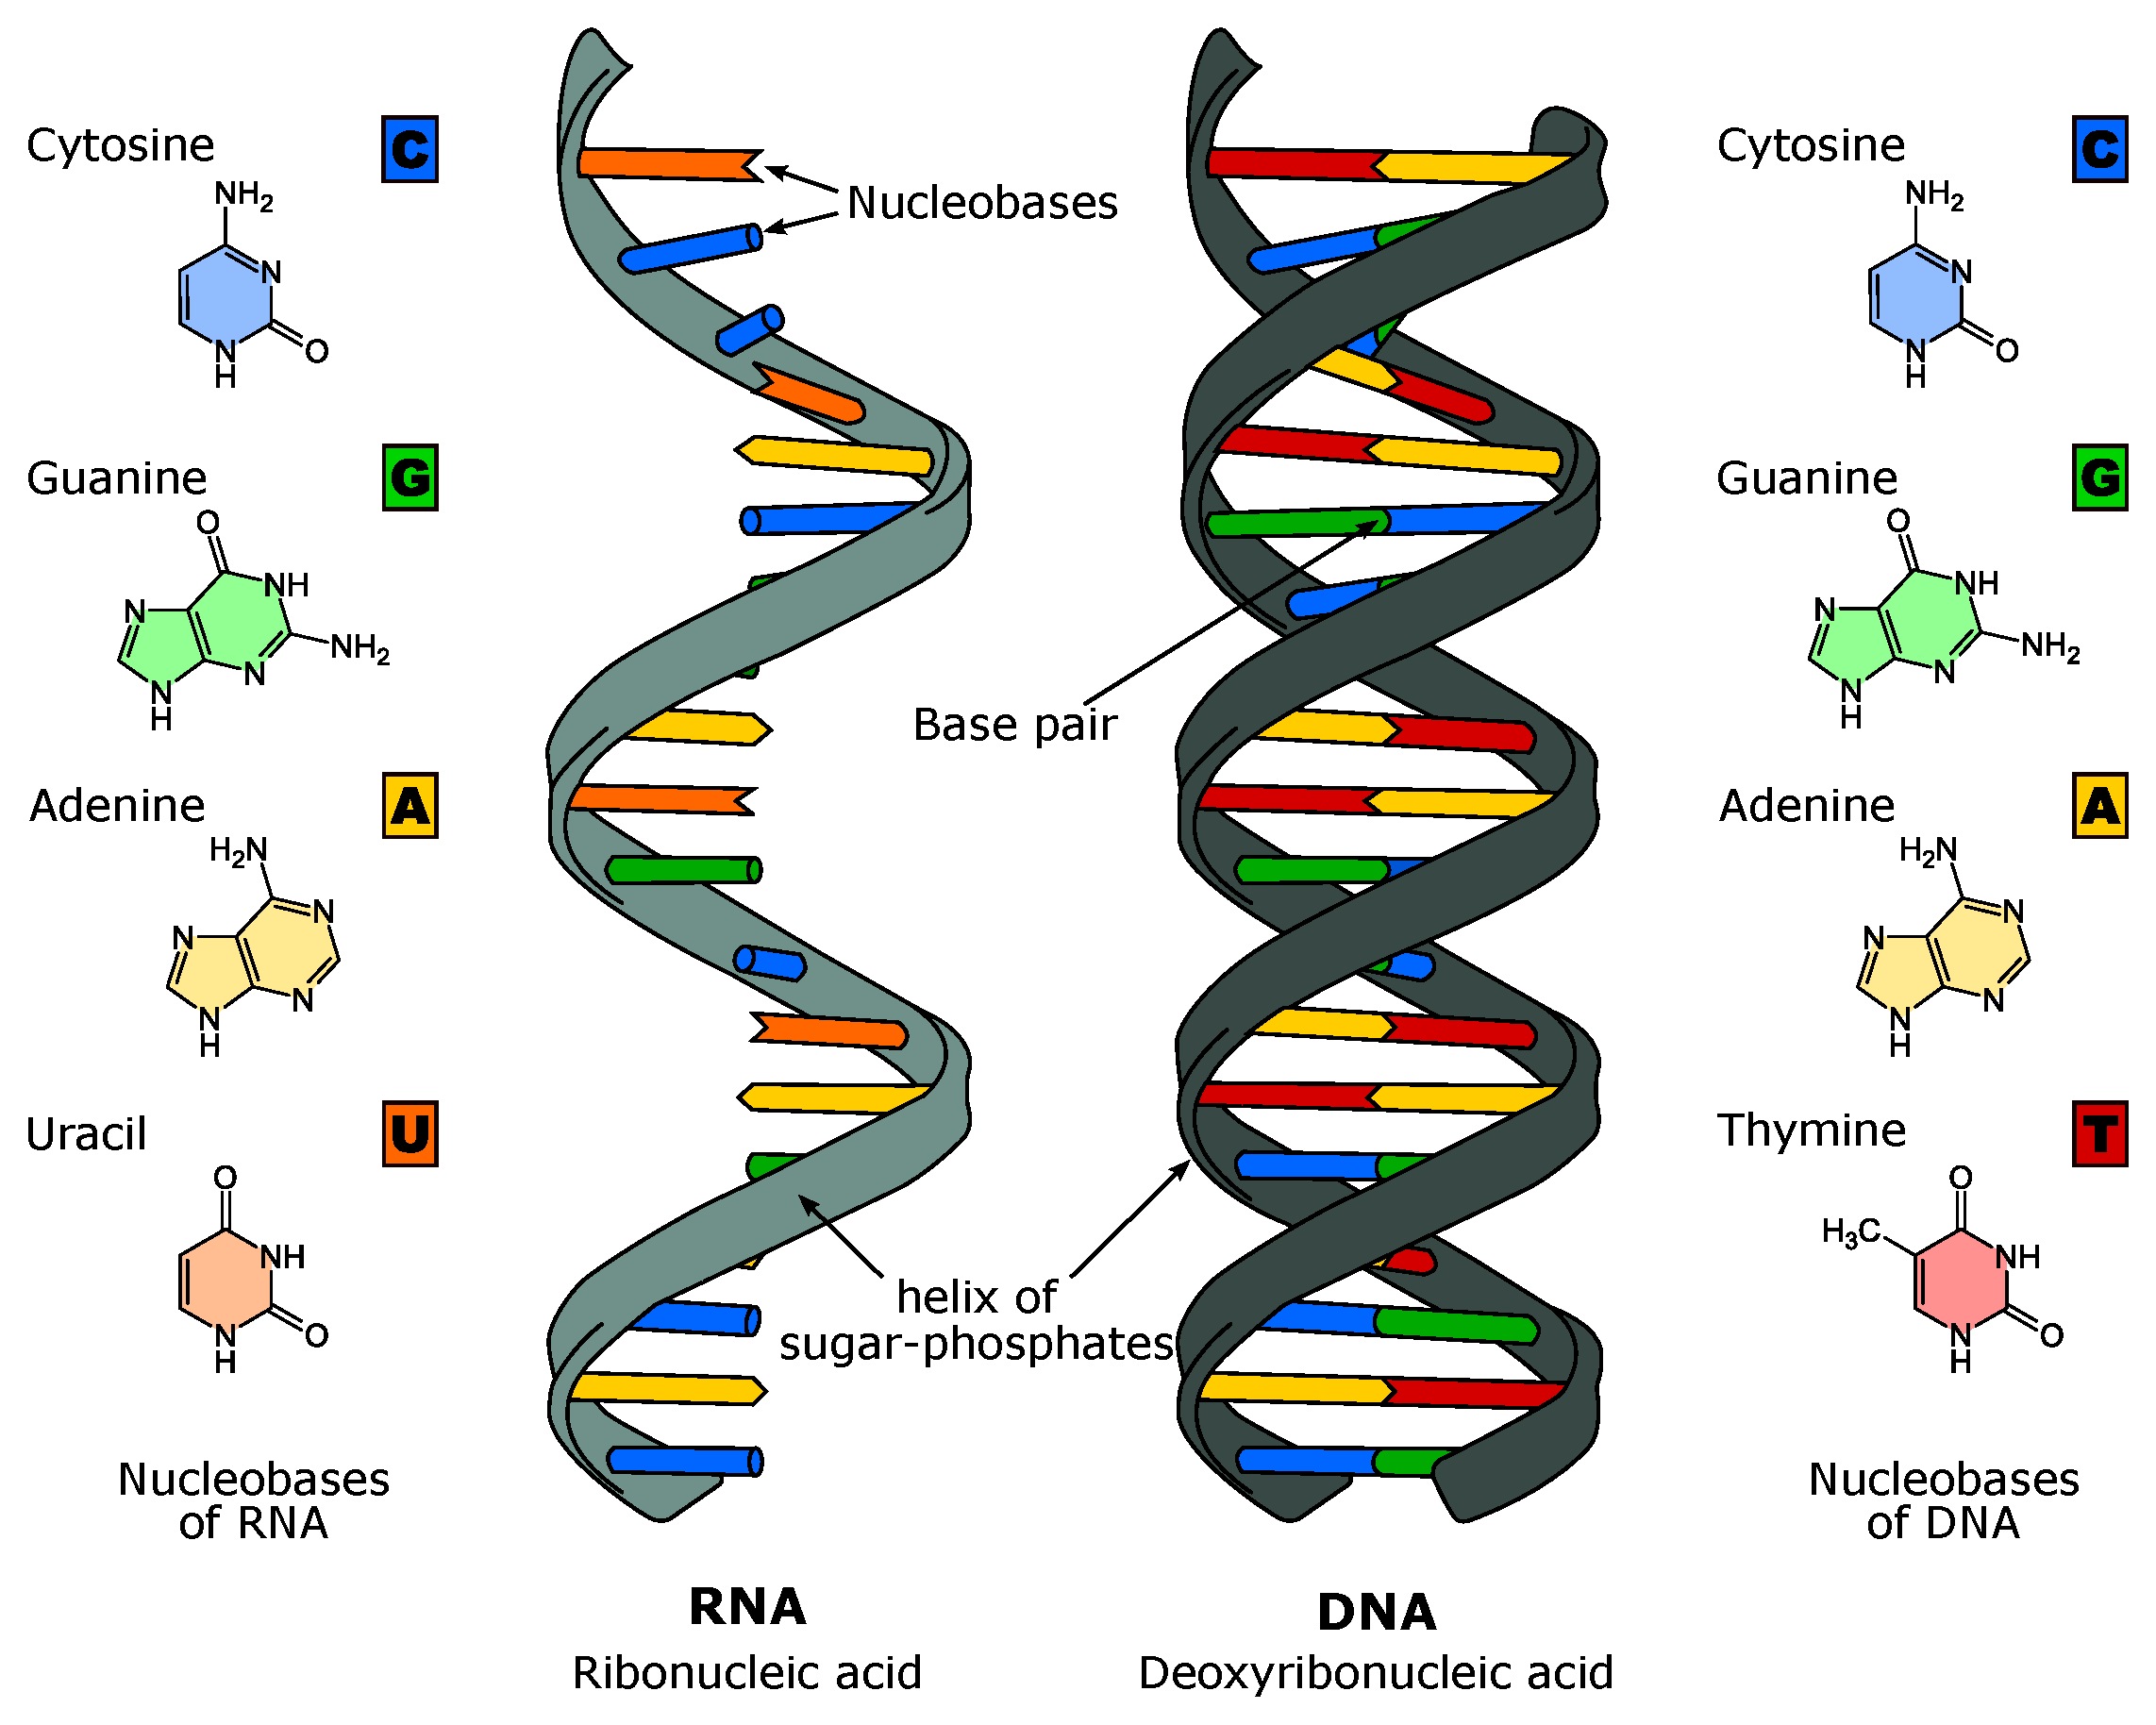
\includegraphics[width=\linewidth]{Difference_DNA_RNA-EN}
		\caption{Structure of DNA and RNA}
		\label{fig:DNA and RNA}
	\end{subfigure}
	~
	\begin{subfigure}{0.34\linewidth}
		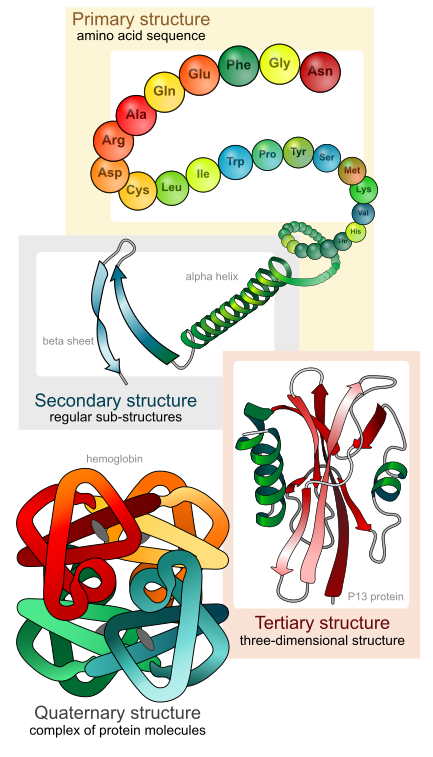
\includegraphics[width=\linewidth]{Main_protein_structure_levels_en}
		\caption{Protein structure}
		\label{fig:protein structure}
	\end{subfigure}
	\caption{Various levels of nucleic acid and peptide structure. Source: Wikipedia.}
\end{figure}

Luckily, at least in the special case of \emph{coiled coil} proteins, we know their 3D structure, and, even more importantly, \cite{potapov2015data} has presented a ``good enough'' method for determining whether two peptide (sub)sequences will form a coiled coil. It will be described in the following section.

The structure of the coiled coils is as follows: Broadly speaking, they look like two helices coiled around each other like two strands of a rope (Figures \ref{subfig:Structure of coiled coils c}, \ref{subfig:Structure of coiled coils d}). However, in order to understand their interactions, we need to describe what happens at the level of individual amino-acids. Namely, due to the circular arrangement of the amino acids around their backbone (Figure \ref{subfig:Structure of coiled coils b}), we obtain what is referred to as the ``knobs into holes packing''. It turns out that the amino acids participating in the inter-peptide interface are located on positions that are congruent to a certain fixed set of numbers modulo 7. That is why we group the amino acids from each peptide into \emph{heptads} -- groups of 7 consecutive amino acids. We denote the positions within the heptads with letters A, B, C, D, E, F, G (for one chain), and A', B', C', D', E', F', G' (for the other).

\begin{figure}[h]
	\centering
	\begin{subfigure}{0.48\linewidth}
		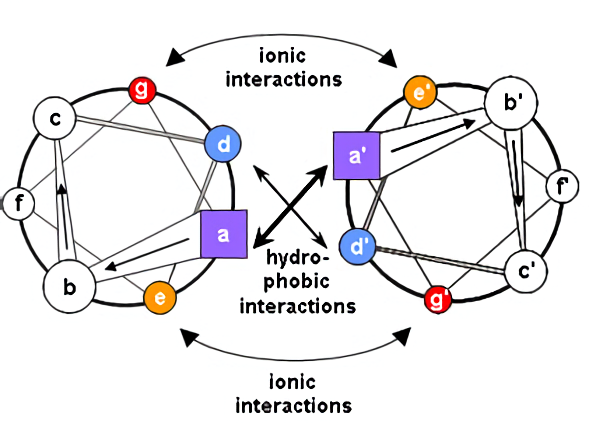
\includegraphics[width=\linewidth]{coiled_coil_structure_a}
		\caption{}
		\label{subfig:Structure of coiled coils a}
	\end{subfigure}
	~
	\begin{subfigure}{0.48\linewidth}
		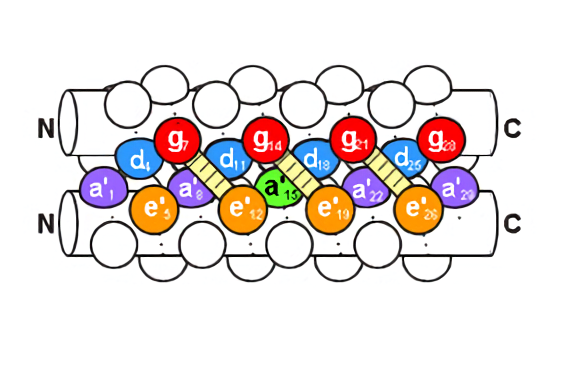
\includegraphics[width=\linewidth]{coiled_coil_structure_b}
		\caption{}
		\label{subfig:Structure of coiled coils b}
	\end{subfigure}
	~
	\begin{subfigure}{0.48\linewidth}
		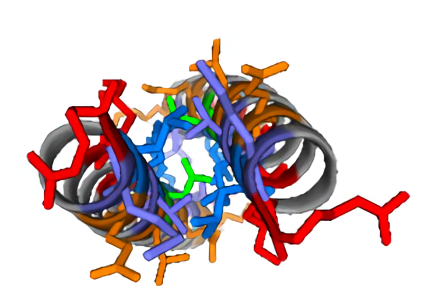
\includegraphics[width=\linewidth]{coiled_coil_structure_c}
		\caption{}
		\label{subfig:Structure of coiled coils c}
	\end{subfigure}
	~
	\begin{subfigure}{0.48\linewidth}
		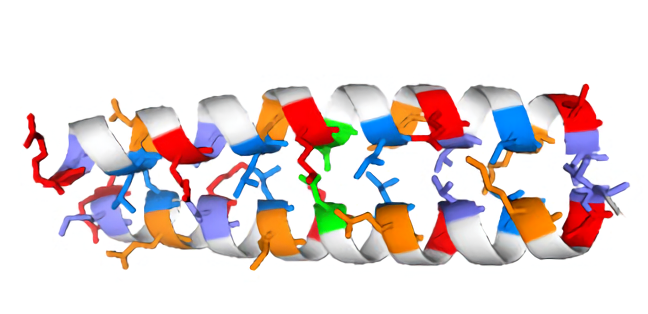
\includegraphics[width=\linewidth]{coiled_coil_structure_d}
		\caption{}
		\label{subfig:Structure of coiled coils d}
	\end{subfigure}
	\caption{The structure of coiled coils. Source: Wikipedia.}
	\label{fig:Structure of coiled coils}
\end{figure}

\section{Scoring function}
\label{sec:Scoring function}

Given this structure, as well as some experimental data, it was reasonable to assume that the interactions within a coiled coil will be governed by the residues at positions A, D, E, G in the heptad, and even then, only if those positions belong to the same, or neighboring heptads (Figures \ref{subfig:Structure of coiled coils a} and \ref{subfig:Structure of coiled coils b}). So, \cite{potapov2015data} described an interaction of two peptides within a coiled coil using a vector $f$ in $\mathbb Z^n$, where each entry represents the number of specific residue pairs and triplets in a given spatial configuration. 

Finally, the authors fitted a linear model based on some experimental data, so we can compute the interaction score as $s = f \cdot w$, where $w$ is the obtained \emph{weight vector}. Thus, the interaction score is the weighted linear combination of the components (``features'') of the \emph{feature vector} $f$.  If we compute the pairwise interaction scores of a set of peptides, we can represent them as a real-valued square matrix, the \emph{interaction matrix}. We will concern ourselves only with peptide sets where every peptide has the same length. Since the scoring function is symmetric with respect to the ordering of its arguments, the obtained matrix is symmetric as well. An example of such a matrix can be seen on Figure \ref{subfig:Interaction matrix of the natural diheptad set}. There, lower (more negative) interaction scores represent stronger binding, and are indicated by darker colors. 

Chemically, the scoring function approximates the base 10 logarithm of the \emph{dissociation constant} $K_d$. For a general reaction 
\begin{align}
A_xB_y \rightleftharpoons xA + yB,
\end{align}
where the complex $A_xB_y$ breaks into $x$ $A$ subunits and $y$ $B$ subunits, the dissociation constant is defined as
\begin{align}
K_d = \frac{[A]^x [B]^y}{[A_xB_y]},
\end{align}
where $[A]$, $[B]$, and $[A_xB_y]$ are the concentrations of $A$, $B$, and the complex $A_xB_y$, respectively. In our case we are just dealing with two peptides that might or might not bind, so $x$ and $y$ become 1, and the definition reduces to $K_d = \frac{[A][B]}{[AB]}$. Now it is clear that the stronger the binding between the peptides $A$ and $B$, the closer $K_d$ is to 0, which implies that the score is more negative for stronger interactions.

\chapter{Previous results}
\thispagestyle{fancy}
\label{chap:Previous results}

Now that we have method for determining whether two sequences interact, the next step is to find a way to fold a long one-dimensional chain into a two- or three-dimensional shape. The first such method was proposed by \cite{gradivsar2013design}. In their paper, Gradišar et al. described some general results about realizing certain graphs (regarded as a wireframe of an object), as well as some experimental results about the construction of a single chain polypeptide tetrahedron, that was built using their algorithmic insights.

In this chapter, we will present some solutions to the following problems:
\begin{enumerate}[(i)]
	\item Define what does it mean for a certain graph to be \emph{realizable} as a peptide chain. \label{item:previous work question 1}
	\item Find some classes of graphs that are realizable using a single peptide chain. \label{item:previous work question 2}
	\item Develop an algorithm for explicitly constructing a peptide chain that will fold into a given graph. \label{item:previous work question 3}
\end{enumerate}

First of all, the original goal set forth by \cite{gradivsar2013design} was to create a rigid 3D object from a single chain. The easiest way to accomplish this (in terms of the ease of synthesis) is to have the peptide laid out along the edges of a polyhedron $P$, covering each edge exactly twice. In graph-theoretical terms, we define the \emph{Eulerian tour} of an arbitrary graph $G=(V, E)$ as a walk in $G$ that visits each edge in $E$ exactly once. Thus, we are looking for the Eulerian tour of the graph $D(P)$ obtained from the polyhedron graph $P$ by duplicating its edges. For brevity, we will sometimes call such a tour the \emph{double trace} of $P$. An example of a double trace of the tetrahedron can be seen on Figure \ref{fig:Tetrahedron process}b).

It turns out that such a setup gives rise to a few additional constraints, which prevent the polyhedron (i.e. the polypeptide chain along its edges) from ``falling apart''. More precisely, let $T$ be the (oriented) Eulerian tour of $D(P)$. Then, the following holds for every vertex $u$ of $D(P)$:
\begin{enumerate}[1)]
	\item After $T$ enters $u$ from a vertex $v$, it does not immediately return to $v$. \label{item:stability constraint 1}
	\item After $T$ passes $u$ as $w\to u \to v$, it later neither passes $u$ as $v\to u \to v$ nor as $w\to u \to v$. \label{item:stability constraint 2}
\end{enumerate}

Every vertex $u$ satisfying the constraints above is called \emph{stable}. Since \ref{item:stability constraint 1}) and \ref{item:stability constraint 2}) are well-defined for the vertices of an arbitrary graph $G=(V, E)$, we say that $G$ is \emph{realizable} if there exists a double trace $T$ of $G$ with respect to which every vertex $v \in V$ is stable.

The forbidden configurations arising from these constraints are also depicted on Figure \ref{fig:Forbidden configurations} below. Although this is not the only way to constrain the ``topology'' of the polypeptide chain, we present it here since it is easy to describe and analyze mathematically, yet good enough for practical applications. The interested reader can see \cite{kovcar2015topofold} for a more thorough discussion of constraining double traces.

\begin{figure}[h]
	\centering
	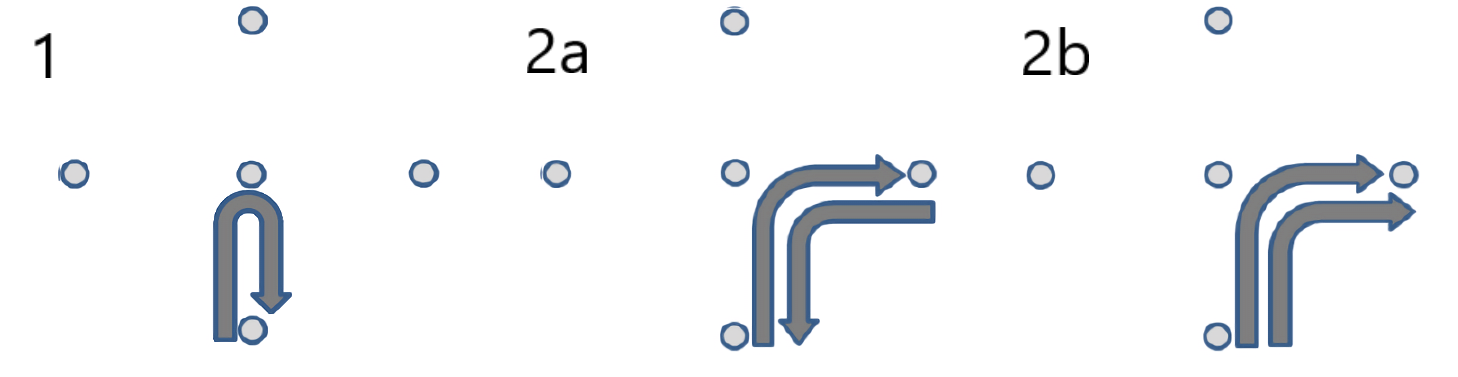
\includegraphics[width=\linewidth]{forbidden_paths.png}
	\caption{Forbidden configurations arising from constraints \ref{item:stability constraint 1}) and \ref{item:stability constraint 2}).}
	\label{fig:Forbidden configurations}
\end{figure}

Note that in this construction the only segments of the peptide chain that are allowed to interact are those that are placed along the same edge of $P$. Moreover, we call two such segments \emph{parallel}, if both corresponding edges of $T$ are oriented in the same way, and \emph{antiparallel} otherwise.
The whole workflow in the specific case of the tetrahedron synthesized by \cite{gradivsar2013design} is depicted on Figure \ref{fig:Tetrahedron process}. 

\begin{figure}[h]
	\centering
	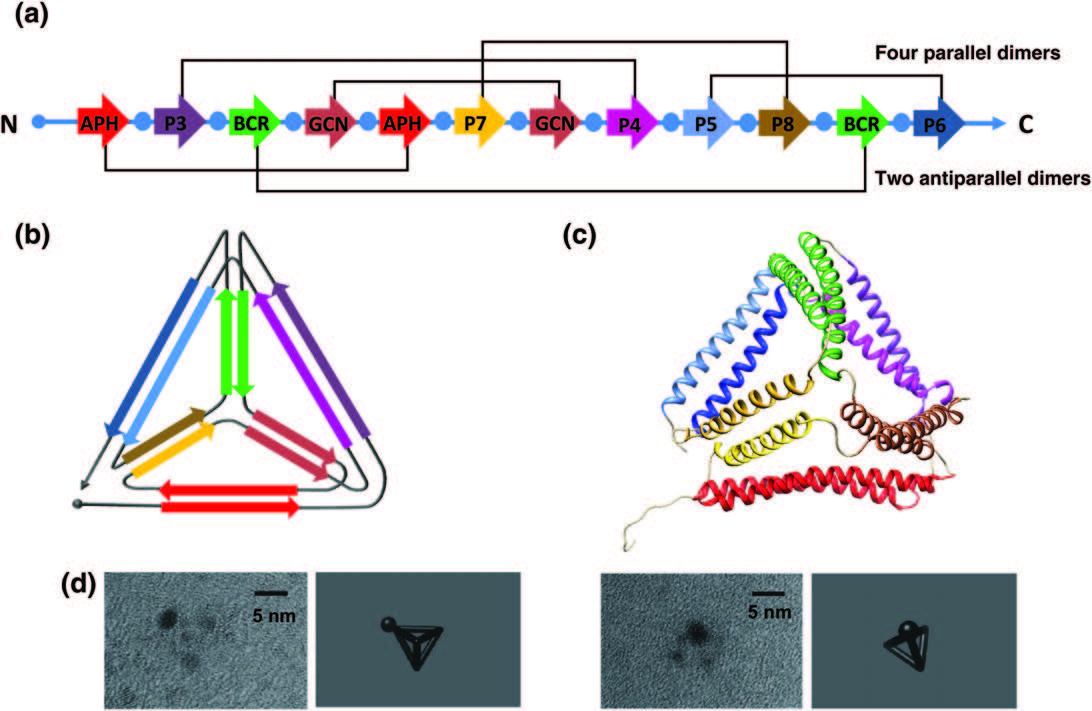
\includegraphics[width=0.8\linewidth]{tetrahedron_process}
	\caption{Rigid tetrahedron being assembled from a polypeptide chain.}
	\label{fig:Tetrahedron process}
\end{figure}

It is clear that we have no reason to restrict ourselves to polyhedron graphs, when discussing their realizability as polypeptide chains. Indeed, for a general graph, we can easily see that it can not contain a vertex of degree 1 or 2, since otherwise constraints \ref{item:stability constraint 1} and \ref{item:stability constraint 2} are not satisfied, respectively. On the other hand \cite{gradivsar2013design} has proved that all cubic graphs (i.e. graphs where all vertices have degree 3) are realizable. The result is proven using the following lemma.

\begin{lemma}
	\label{lemma: cubic}
	Let $G$ be a graph, and $T$ its double trace, that is, the Eulerian tour of $D(G)$. Let $u$ be a vertex of degree 3 in $G$. Then, $u$ is stable (with respect to $T$) if and only if condition (i) is fulfilled for $u$.
\end{lemma}

The proof of the lemma is straightforward. Now, we can prove the main theorem in this chapter, giving us a partial solution to problem (\ref{item:previous work question 2}) from the beginning of this chapter.

\begin{theorem}
	All connected cubic graphs are realizable.
\end{theorem}

\begin{proof}
	Let $G = (V, E)$ be a cubic graph with $m$ edges, and $G' = D(G)$ its double. Recall that $G'$ is constructed from $G$ by adding to $E$ a new edge $e'$ parallel to $e$, for every $e \in E$. Call consecutive arcs of an Eulerian tour that traverse $e$ and $e'$ (for some $e \in E$) one after the other a \emph{bad pair}. By lemma \ref{lemma: cubic} we just need to show that $G'$ admits an Eulerian tour without bad pairs. In fact, since all vertices of $G'$ have an even degree (6), we know that $G'$ does contain an Eulerian tour $T$, 
	\begin{align} T = v_1 \rightarrow v_2 \rightarrow \dots \rightarrow v_{2m} \rightarrow v_1.
	\end{align}
	Let $s$ be the number of bad pairs. Without loss of generality, we may assume that $s\geq 1$, because otherwise there is nothing to be proven. Also, we can label the vertices of $T$ such that $T$ starts with $v_1 \rightarrow v_2 \rightarrow v_3 = v_1 \rightarrow\dots$, i.e. that $(v_1v_2,\;v_2v_3)$ is the first bad pair. We know that since $v_2$ has degree at least 2 in $G$, there exists an index $i \geq 3$ for which $v_i = v_2$. Take the smallest such index. Observe also that $i \geq 5$ and $v_{i+1}\notin \{v_1, v_2\}$. Now, we can get rid of the bad pair $v_1 \rightarrow v_2 \rightarrow v_3 = v_1$ by defining a new Eulerian tour $T'$ with
	\begin{align}
	\begin{split}
	T' &= v_1 \rightarrow v_2 \rightarrow v_{i-1} \rightarrow v_{i-2} \rightarrow \dots \rightarrow v_4 \rightarrow \\ &\rightarrow v_1 \rightarrow v_2 \rightarrow v_{i+1} \rightarrow v_{i+2} \rightarrow \dots \rightarrow v_{2m} \rightarrow v_1.
	\end{split}  
	\end{align}
	
	We also see that the second occurrence of $v_1 \rightarrow v_2$ does not form a bad pair with either of $v_2 \rightarrow v_{i+1}$ or $v_4 \rightarrow v_1$. Since these are the only bad pairs we might have introduced, and we have removed at least one from $T$, it follows that $T'$ has at most $s-1$ bad pairs. Repeating this procedure, we obtain an Eulerian tour with no bad pairs.
\end{proof}

Finally, the only remaining question is about the algorithm for explicitly constructing a peptide chain that will actually realize the given graph. As it was mentioned earlier, for that we need to create many pairs of peptides that will interact only mutually. Later on, we will call such a set of peptide-pairs an \emph{orthogonal set}. Once we have such a set, we can concatenate the peptides in the order orientation determined by the double trace of the graph. Two methods for constructing such a set will be given in sections \ref{sec:exact-algorithm} and \ref{sec:heuristics}.

\chapter{Computational complexity}
\thispagestyle{fancy}
\label{chap:Computational complexity}

Before presenting any further algorithms that are directly related to our end goal, we need to define what makes an algorithm fast and efficient, versus slow, and even infeasible. The area of mathematics and computer science that addresses this, and many other questions is called \emph{computational complexity theory}. In this chapter we will present a small subset of the theory, needed to understand the complexity classes $\P$, $\NP$, and their relatives.  

The naive way to quantify the efficiency of an algorithm would be to run the algorithm for a certain input, and measure its execution time using a stopwatch. However, this approach has a many obvious drawbacks: we have no idea how the algorithm would perform when given any other input, we have no way of predicting how fast would it run on another machine, we have no way of comparing it to any other algorithm, possibly running on another machine\dots This clearly implies the need for a framework that will predict how quickly would the running time increase as a function of the input size. Of course, the running time is just an example metric, and the theory could be generalized to others, such as memory usage, or the number of times a certain resource is accessed.

The starting point of complexity theory is the definition of the \emph{Turing machine}, developed by Alan Turing in 1936, in order to formalize the notions of algorithms, computability and decidability.

\begin{definition}
	A \emph{Turing machine} is a tuple $ ( Q, \Gamma, \Sigma, q_0, b, F, \tau)$, where
	\begin{itemize}
		\item $Q$ is the set of \emph{states},
		\item $\Gamma$ is the set of \emph{tape symbols},
		\item $\Sigma \subset \Gamma$ is the set of \emph{input symbols}, 
		\item $q_0$ is the initial state,
		\item $b \in \Gamma \backslash \Sigma$ is the special \emph{blank symbol},
		\item $F \subset Q$ is the set of \emph{accepting states},
		\item $\tau: Q \times (\Gamma \cup \{b\}) \to Q \times \Gamma \times \left \{ L, R \right \}$ is the \emph{transition function}. It is important to note that $\tau$ can be a partial function, that is, it does not need to be defined everywhere on $Q \times \Gamma$.
	\end{itemize}
\end{definition}	

Having this definition, we still need to specify how a Turing machine operates: First of all, the Turing machine has at its disposal an infinite tape of cells, filled with symbols from $\Gamma$. Initially, first $n$ cells of the tape are filled with symbols from $\Sigma$ (this is the \emph{input} to the Turing machine), while the remaining cells contain $b$. Besides the tape, a Turing machine is associated with its current state $q \in Q$ (which is equal to $q_0$ at the beginning), and the position of its \emph{read-write head} on the tape. Once set up, the Turing machine performs a (possibly) sequence of steps by reading the current symbol from the tape, writing a symbol and changing its state based on the transition function, and finally moving its head left or right, depending on whether the last component of the transition tuple is $L$ or $R$. 

If, for a given input, the machine can not perform a transition (i.e. if $\tau$ is not defined for the current state and tape symbol), we say that it \emph{halts}. If, additionally, the machine halts in an accepting state, we say that it has \emph{accepted} the input.
The set of all inputs accepted by a Turing machine $M$ is the \emph{language} of that machine, and is denoted by $L(M)$. From now on, we will only be interested in Turing machines that halt after a finite number of steps for all possible inputs. In particular, we will be looking for an upper bound on how quickly that number increases as a function of input size.

It turns out that such a Turing machine captures the essence of our informal understanding an algorithm as a finite decision procedure. More specifically, we define a \emph{decision problem} for a set $A \subseteq \Sigma ^*$ (here, $\Sigma^*$ for any set $\Sigma$ denotes the set of all finite-length strings composed from elements of $\Sigma$) as the problem of determining whether a given word $w \in \Sigma ^*$ belongs to $A$. Then, an algorithm for that problem is just a Turing machine $M$ with $L(M) = A$. In that case we say that $M$ \emph{decides} $A$. Sometimes, we might also treat $M$ itself as the \emph{characteristic function} of $A$, that is, as a function $M: \Sigma ^* \to \{0, 1\}$ for which
\begin{align}
	M(x) = \begin{cases}
		1 & \text{if } x \in A, \\
		0 & \text{otherwise.}
	\end{cases}
\end{align}

Given the definitions above, now it is a good time to define our first two complexity classes, $\DTIME$, and $\P$.

\begin{definition}
	Let $T:\mathbb N \to \mathbb N$ be some function. A language $L$ is in $\DTIME(T(n))$ iff there is a Turing machine that does at most $c \cdot T(n)$ steps for some constant $c > 0$ and decides $L$.
\end{definition}

\begin{definition}
	 The class $\P$ is defined as
	 \begin{align}
	 	\P = \bigcup_{c\geq 1} \DTIME (n^c).
	 \end{align}
\end{definition}

Although the class of decision problems seems too simple, we can in fact build layers of abstractions that will allow us to describe complex input objects. For example, first we decide that we will encode integers as their binary representations, then we use that to encode sequences and matrices, and finally we represent arbitrary graphs using their adjacency matrices. We will assume that such an encoding exists for all ``interesting'' mathematical objects. The cost of these abstraction incurs at most a polynomial penalty in the running time. Furthermore, we may extend our basic definition of the Turing machine with many convenient extensions such as multiple tapes, and these extensions come again at a polynomial increase in the number of the performed steps \cite{arora2009computational}. In particular, we can allow a Turing machine to take multiple mathematical objects as its input, by encoding them as strings from $\Sigma^*$, and separating them with a single blank symbol $b$ on the input tape. More formally, that Turing machine can now be regarded as the characteristic function of the set $A_1 \times A_2 \times \dots \times A_k$, where $A_i$ are some sets whose elements can be encoded as strings from $\Sigma^*$.

The above reasoning implies that, in fact, the choice of the exact computational model is largely unimportant, if we are willing to allow a polynomial slowdown. That is to say that, if a problem is solvable in a polynomial number of steps using some deterministic computational system, it can also be solved by a Turing machine in polynomial time (i.e. it belongs to $\P$). Finally, it is widely agreed that $\P$ is the class of decision problems with efficient decision procedures. Although it can be argued whether a class such as $\DTIME(n^{100})$ represents feasible real world computation, very few problems are known to intrinsically require a high-exponent polynomial solution. One well-known example of such an algorithm is the original version of the AKS deterministic primality test, which was originally reported as $O(n^{12})$ \cite{agrawal2004primes}, however it was soon improved to $O(n^6)$ in \cite{lenstra2002primality}. 

In contrast to $\P$, which turned out to be the class of efficiently solvable decision problems, we will now proceed to define $\NP$, the class of decision problems whose solutions can (just) be easily verified. Following the definition of $\P$, we will require the verification process to take at most a polynomial (in the size of the input) amount of time.

\begin{definition}
	\label{def: First NP definition}
	A language $L \subseteq \{0, 1\}^*$ is in $\NP$ if there exists a polynomial $p : \mathbb N \to \mathbb N$ and a polynomial-time Turing machine $M$ (called the \emph{verifier} for $L$) such that for every $x \in \{0, 1\}^*$,
	\begin{align} 
	x\in L\Leftrightarrow \exists u \in \{0, 1\}^{p(|x|)} \text{ such that } M(x, u) = 1
	\end{align}
	If $x\in L$ and $u \in \{0, 1\}^{p(|x|)}$ satisfy $M(x, u) = 1$, then we call $u$ a \emph{certificate} for $x$ (with respect to the language $L$ and machine $M$).
\end{definition}
It follows trivially that every problem in $\P$ is also in $\NP$, since the certificate can be the empty string, and the verifier the Turing machine that decides that problem. There also exists an equivalent definition of $\NP$, which uses the concept of a \emph{nondeterministic} Turing machine:

\begin{definition}
	A \emph{nondeterministic Turing machine} is a Turing machine $M = ( Q, \Gamma,\allowbreak \Sigma,\allowbreak q_0,\allowbreak b, F, \{\tau_0, \tau_1\})$ with two transition functions $\tau_0, \tau_1$ which at every step makes an arbitrary choice about which transition function to apply. 
	
	Consequently, $M(x)=1$ for some input $x$, if there exists some sequence of the choices of the transition function for which $M$ accepts $x$. Otherwise, if for every sequence of choices $M$ halts without accepting $x$, we say that $M(x) = 0$.
\end{definition}

Analogously to $\DTIME(T(n))$, we define $\NTIME(T(n))$ in the following way:

\begin{definition}
	For every function $T: \mathbb N \to \mathbb N$ and $L \subseteq \{ 0, 1 \}^*$, we say that $L \in \NTIME(T(n))$ if there is a constant $c > 0$ and a $cT(n)$-time nondeterministic Turing machine $M$ such that for every $x\in \{0, 1\}^*$, $x\in L \Leftrightarrow M(x) = 1$.
\end{definition}

Finally, we can state the alternative definition of $\NP$:

\begin{definition}
	\begin{align}
	\NP = \bigcup_{c \in \mathbb N} \NTIME(n^c).
	\end{align}
\end{definition}

The proof of the equivalence of the two definition stems from the fact that the sequence of choices between the two transition functions can be regarded as a certificate in the definition \ref{def: First NP definition}.
In any case, the following are some examples of well-known decision problems that belong to $\NP$:
\begin{description}
	\item[Independent set problem] This is the set (language) of all pairs $(G, k)$, where $G$ is a graph containing a subset of at least $k$ vertices with no edges between them. Alternatively, when given an arbitrary graph $G$ and a natural number $k$, we interpret the question of language membership as ``Does $G$ contain a subset $S$ of at least $k$ vertices with no edges between them?''. A polynomial size certificate would be a binary vector $u$ of length equal to the number of vertices in $G$, representing characteristic function of $S$.
	\item[Subset sum] Given a list of $n$ numbers $a_1,\dots,a_n$ and a number $T$, decide if there
	is a subset of the numbers that sums up to $T$. The certificate is the list of members
	in such a subset.
	\item[Compositeness testing] Given a number $N$ decide if $N$ is a composite (i.e., non-prime)
	number. The certificate are two nontrivial factors of $N$.
	\item[Connectivity] Given a graph $G$ and two vertices $s, t$ in $G$, decide if $s$ is connected to
	$t$ in $G$. The certificate is a path from $s$ to $t$.
\end{description}

The last two problems in this list (compositeness/primality testing and connectivity) are also known to be in $\P$. For first two problems, however, it turns out that they are as hard as the hardest problems in $\NP$, and thus not in $\P$ unless $\P = \NP$.

The question of whether $\P = \NP$ is in fact one of the central questions in computational complexity theory. In fact, many other complexity classes were developed in order to help us to better understand the relation between $\P$ and $\NP$. The two possible relations are shown on Figure \ref{fig: P vs NP}. The following definitions will define some of these classes, and formalize the notion of one problem being \emph{at least as hard as} some other problem.

\begin{definition}
	A language $L \subseteq \{0, 1\}^*$ is \emph{polynomial-time Karp reducible} to a language $L'\subseteq \{0, 1\}^*$ (or just ``polynomial-time reducible''), denoted by $L \leq_p L'$, if there is
	a polynomial-time computable function $f : \{0, 1\}^* \to \{0, 1\}^*$ such that for every
	$x \in \{0, 1\}^*$, $x\in L$ if and only if $f(x) \in L'$.
	
	We say that $L'$ is $\NP$-hard if $L \leq_p L'$ for every $L \in \NP$. We say that $L'$ is
	$\NP$-complete if $L'$ is $\NP$-hard and $L' \in \NP$.
\end{definition}

Informally, we understand that $L \leq_p L'$ means that $L'$ is as hard as (if not harder than) $L$. 
Thus, most often, proving that a language is $\NP$-complete, amounts to finding a polynomial time verifier to prove that it is in $\NP$, and reducing a known $\NP$-complete problem to it, in order to prove that it is $\NP$-hard, and, therefore $\NP$-complete. The original list of $\NP$-complete problems was given by Karp in \cite{karp1972reducibility}, but it has been subsequently expanded by \cite{gary1979computers}.

\begin{figure}[h]
	\centering
	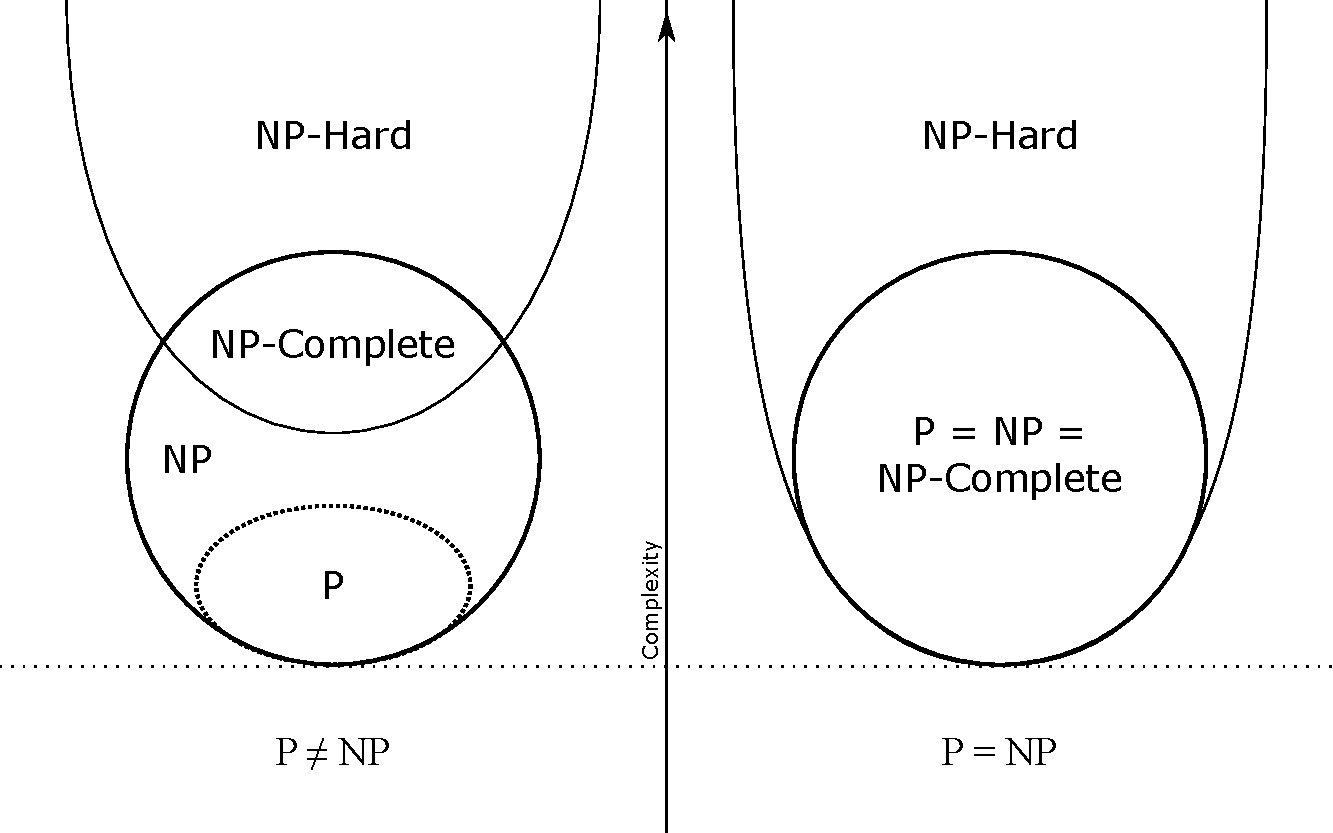
\includegraphics[width=0.8\linewidth]{P_vs_NP}
	\caption{Two possible relations between $\P$ and $\NP$.}
	\label{fig: P vs NP}
\end{figure}

\chapter{Orthogonal sets}
\thispagestyle{fancy}
\label{chap:Orthogonal sets}

\section{Definition and $\NP$-completeness}

Recall from the end of chapter \ref{chap:Previous results} that we needed to construct a large set of peptide-pairs that interact only mutually (an \emph{orthogonal set}). The most straightforward (and most general) approach is to search for such a set as a subset of some larger set of all admissible peptides. 

Also, since the scoring function (introduced in section \ref{sec:Scoring function}) is just an approximation of the underlying chemical processes, we need a robust way of defining whether two peptides interact. In order to do that, we introduce two thresholds for the interaction score, with a ``safety zone'' between them. The following definitions formalize these notions.

 
\begin{definition}[Interaction types]
	Let $A$ be a set of peptides (\emph{admissible set}), and $M$ its interaction matrix, as defined in section \ref{sec:Scoring function}.
	Let $c_s$ and $c_w$ be two real numbers with $c_s < c_w$. Then, for a peptide pair $i, j\in A$ with interaction score $M_{ij}$ we have the following:
	\begin{enumerate}[a)]
		\item If $M_{ij} > c_w$, we say that $i$ and $j$ are \emph{not interacting};
		\item If $M_{ij} \leq c_w$, we say that $i$ and $j$ are \emph{interacting};
		\item If $i$ and $j$ are interacting, and $M_{ij} \leq c_s$, we say that they are \emph{strongly interacting}.
	\end{enumerate}
\end{definition}

\begin{definition}[Interaction graph]
	Let $A$, $M$, $c_s$, $c_w$ be as in the previous definition.
	The (undirected) \emph{interaction graph} of $A$ with respect to $c_s$ and $c_w$ is the 3-tuple $G_i = (V, E, E_s)$, where 
	\begin{enumerate}[i)]
		\item $V = A$ (the set of peptides);
		\item $E = \{ \{i, j\} | M_{ij} \leq c_w \}$ (the set of all interacting peptide-pairs) 
		\item $E_s = \{ \{i, j\} | M_{ij} \leq c_s \}$ (the set of all strongly interacting peptide-pairs/edges)
	\end{enumerate}
\end{definition}

\begin{definition}[Orthogonal set]
	Let $G=(V, E)$ be a graph, and $E_s \subseteq E$. A subset $S \subseteq E_s$ is an \emph{orthogonal set} if for any two distinct edges $u_1v_1, u_2v_2 \in S$ the following holds:
	\begin{enumerate}[i)]
		\item The two edges are not incident to each other, i.e. $\{u_1,v_1\} \cap \{u_2, v_2\} = \emptyset.$
		\item The two edges are not incident to a common edge, that is, \[\{u_1u_2,\; u_1v_2,\; v_1u_2,\; v_1v_2\} \cap E = \emptyset.\]
		\item Additionally, if $u_1 \neq v_1$ (i.e. the edge is not a loop), we require that $u_1$ and $v_1$ are not incident to any loops in $E$. 
	\end{enumerate}
	\label{def:Orthogonal set}
\end{definition}

An alternative way to define orthogonal sets uses the notion of a \emph{line graph}.
\begin{definition}[Line graph]
	Let $G$ be a graph. The \emph{line graph} of $G$, denoted as $L(G)$ is the graph whose vertices correspond to edges of $G$, and are connected if their corresponding edges in $G$ are incident to each other.
\end{definition}

\begin{proposition}[Alternative definition of an orthogonal set]
	Let $G = (V, E)$ be a graph, and $E_s \subseteq E$. Let $L(G) = (E, F)$ be the line graph of $G$. Then, orthogonal sets in $G$ (with respect to $E_s$) correspond to independent subsets of $E_s$ in $L(G)$, where no two vertices share a common neighbor in $L(G)$.
\end{proposition}
In both cases, we see that the orthogonal set is defined with respect to a graph $G=(V, E)$ and a set $E_s \subseteq E$. In our case, we will apply the general results below to interaction graphs $G_i$, where $E_s$ is the set of strongly interacting peptide-pairs.

In accordance to the definition of the maximum independent set, we define the \emph{maximum orthogonal set} as an (as there can be more than one) orthogonal set of maximum cardinality. Continuing the analogy with independent sets, we will be interested in determining, or at least approximating, the maximum orthogonal sets. Before doing that, we will first prove that the maximum orthogonal set problem is $\NP$-complete. In order to use the framework developed in chapter \ref{chap:Computational complexity}, we need to phrase it as a decision problem -- the \emph{orthogonal set problem}.

\begin{definition}[Orthogonal set problem]
	Given a graph $G = (V, E)$, a set $E_s \subseteq E$, and an integer $k$, determine whether there exists an orthogonal set of size at least $k$. We denote an instance of the orthogonal set problem as the 4-tuple $(V, E, E_s, k)$.
\end{definition}
From this definition, we immediately obtain the fact that the orthogonal set problem is in $\NP$, since, given any set we can verify in polynomial time whether it is orthogonal, and has cardinality at least $k$. Once we show that this problem is $\NP$-hard, we will get that it is $\NP$-complete.

\begin{theorem}
	The orthogonal set problem is $\NP$-hard.
\end{theorem}
\begin{proof}
	We will prove this by reducing the maximum independent set problem to the maximum orthogonal set problem. Let $G=(V, E)$ be a graph in which we want to determine whether it has an independent set of size at least $k$. Construct a new graph $G'=(V', E')$ from $G$ by adding to $V$ a new vertex $v'$ (the ``copy'' of $v$) for every $v \in V$ and connecting each $v \in V$ to its corresponding copy $v'$. 
	
	Now, let $(V', E', E', k)$ be an instance of the maximum orthogonal set problem (i.e. until the end of the proof, $E_s = E'$). We will prove that the obtained maximum orthogonal set $S$ consists exactly of edges of the form $vv'$, where $v\in V$ and $v'$ is the copy of $v$.
	
	Assume the opposite, i.e. that there exists a pair $u_1v_1 \in S$ which is not of the form $ww'$ for $w \in V$. Then for all $u_2v_2 \in S$ we have $u_1u_2 \notin E'$, $u_1v_2 \notin E'$, $v_1u_2 \notin E'$ and $v_1v_2 \notin E'$. Thus, we can remove $u_1v_1$ from $S$ and replace it with $u_1u_1'$ and $v_1v_1'$ to obtain a larger orthogonal set. Therefore, we have obtained an orthogonal set with more than $|S|$ elements, which is a contradiction.
	
	Using this, we can prove that there exists an independent set $I$ in $G$ with $|I| \geq k$ if and only if there exists an orthogonal set $S$ in $G'$ with $|S| \geq k$ as follows.
	
	\begin{description}
		\item[$(\Rightarrow)$] Let $I$ be an independent set of size $k$ in $G$. Then it is easy to see that $S = \{ vv'| v \in I \}$ is an orthogonal set of the same size in $G'$.
		\item[$(\Leftarrow)$] Let $S$ be an orthogonal set of size $k$ in $G'$. Then there exists a maximum orthogonal set $S_\text{max}$ in $G'$, with size at least $k$. Since $S_\text{max}$ consists only of edges of the form $vv'$, $v \in V$, we can construct an independent set $I = \{ v | vv' \in S_\text{max} \}$, for which $|I| \geq |S_\text{max}| \geq |S| = k$.
	\end{description}

	The argument above completes the reduction of the independent set problem to the orthogonal set problem, and therefore the orthogonal set problem is $\NP$-hard.
\end{proof}

\section{Exact algorithm}\label{sec:exact-algorithm}
Although the previous section gave us a proof that we can not hope (unless $\P=\NP$) to have an efficient algorithm for determining the maximum orthogonal set in a given graph, we can still look for practically efficient algorithms. It turns out that such an algorithm exists, and is based on the line graph definition of an orthogonal set.

We start with a graph $G = (V, E)$ and a set $E_s \subseteq E$ with respect to which we want to determine the maximum orthogonal set. First, from $E_s$ remove all pairs $uv$ where $u \neq v$ and $u$ or $v$ is incident to a loop. Then, form a new graph $G' = (E_s, E')$, where we connect two vertices $u_1v_1$ and $u_2v_2$ if they can not be together in an orthogonal set, i.e. if they do not satisfy the conditions from definition \ref{def:Orthogonal set}.
Finally, we find the maximum independent set in $G'$, which is, by construction the maximum orthogonal set in $G$.

Alternatively, since $G'$ is sparse, we might leverage the state of the art maximum clique algorithms such as \cite{depolli2013exact}, \cite{san2013improved}, or \cite{tomita2010simple} to find the maximum clique in the complement of $G'$. The algorithm we used was from \cite{depolli2013exact}, and it is based on greedily coloring the subgraphs of the given graph, as a means of determining the upper bound for the size of the maximum clique in those subgraphs.

Now that we have described the algorithm, in order to apply it to our case of interaction graphs, we need to describe how to obtain $A$, the set of all admissible peptides. Also, we need to determine $c_w$ and $c_s$, the thresholds that will be used for constructing the interaction graph. 

The answer to the latter is straightforward: Since the scoring function approximates the logarithm of the dissociation constant, we may simply fix the difference $c_w-c_s$ to 1, since that gives us a 10-fold difference in the dissociation constants for the on- and off-target interactions. This amount was suggested by our experimental collaborators, and it can be tuned at the time of synthesis. Furthermore, our own experiments have indicated that the size of the maximum orthogonal set is robust with respect to small changes in $c_w - c_s$.

Once we fix the difference, use the following algorithm to determine the best cutoffs.
\begin{enumerate}
	\item Let $M$ be the interaction matrix of $A$, and $c_\mathrm{min}$ and $c_\mathrm{max}$ its minimum and maximum entries, respectively. Choose $\Delta$ as a small number, relative to $|c_\mathrm{max} - c_\mathrm{min}|$.
	\item For $c_s$ in $\{ c_\mathrm{min},\; c_\mathrm{min} + \Delta,\; c_\mathrm{min} + 2\Delta,\; \dots, c_\mathrm{max} \}$ run the orthogonal set algorithm on the interaction graph of $A$ with respect to the thresholds $c_s$ and $c_w = c_s + 1$. If the algorithm exceeds a predetermined time limit, interrupt it after the time has expired. In any case, save the best obtained results for every pair of cutoffs.
	\item Choose the cutoffs that gave the largest orthogonal set size in the previous step.
\end{enumerate}

Once the best such thresholds are chosen, the algorithm is rerun without time limits. We call the threshold chosen in this way the \emph{recommended threshold}. From now on, we will assume that the used threshold is the recommended one, unless otherwise stated. This approach is reasonable, since although we might interrupt the orthogonal set/maximum clique search before it finds the maximum clique, our experimental data suggests that the size of the clique found after a fixed time is a strong indication for the size of the maximum clique. An example of this process can be seen on Figure \ref{fig:Cutoff bruteforce}.

\begin{figure}[h]
	\centering
	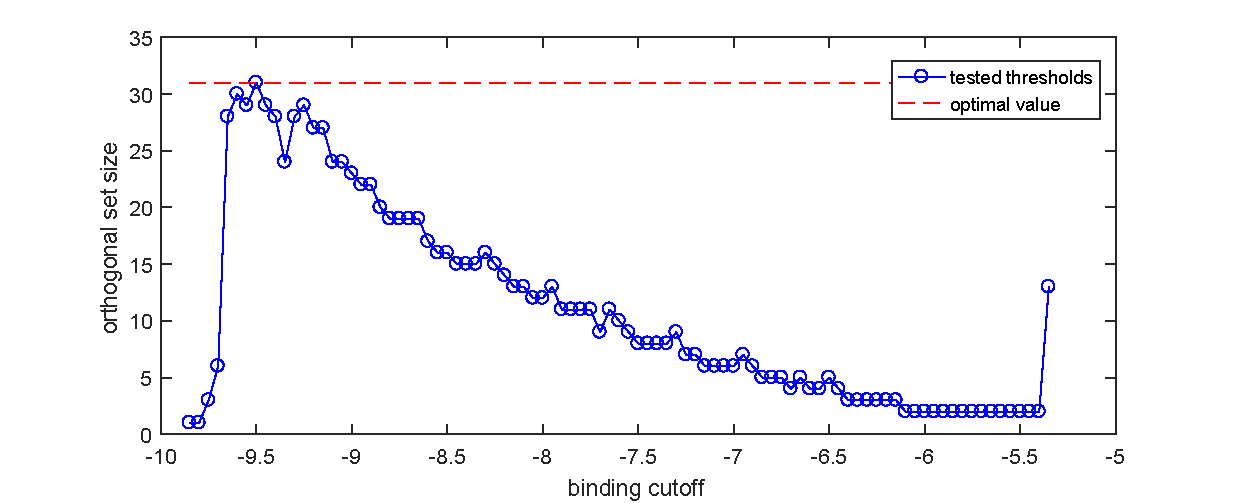
\includegraphics[width=\linewidth]{cutoff_bruteforce.pdf}
	\caption{Orthogonal set sizes for different values of $c_s$, with $c_w-c_s = 1$ and $\Delta = 0.05$.}
	\label{fig:Cutoff bruteforce}
\end{figure}

The answer to the former question (about choosing the right set of admissible peptides) turned out to be an unexpected bottleneck. Since the number of all peptides of a given length grows exponentially with the length, we need to devise a good strategy for reducing the search space, while still having a good sample. The first approach was to determine a suitable set of heptads, and let the initial set be the set of all concatenated $k$-tuples of these heptads. Unfortunately, this approach quickly becomes infeasible for longer peptides and larger heptad sets. Namely, if we have $h$ heptads, there are obviously $h^k$ $k-$heptad peptides that can be built from them. In our algorithm, every pair of peptides can possibly belong to the orthogonal set ($h^{2k}$ pairs), and every two pairs have to be checked for mutual interaction ($h^{4k}$ interactions). Therefore, even when we ignore the cost of the maximum clique computation, and restrict ourselves to 4 or 5 heptads, we see that the approach above is only feasible for very small initial heptad sets.

Although the reasoning above rules out the set of natural heptads (i.e. the set of 1176 heptads occurring in natural coiled coils), the insight from \cite{potapov2015data} and earlier work permits us to consider a set of just 8 ``synthetic'' heptads that cover for the most significant variations observed in nature. The resulting initial set has $8^4 = 4096$ peptides, and the clique search is ran on 1650 vertices (peptide pairs). Using the recommended threshold, we obtain a 35-peptide orthogonal set with 23 homodimers and 12 heterodimers. Their interaction matrix can be seen on Figure \ref{fig:interaction matrix-full4096}. In particular, note the dark (block-)diagonal, which represents strong interactions between peptides -- in each row and column there exists exactly one such field.

\begin{figure}[h]
	\centering
	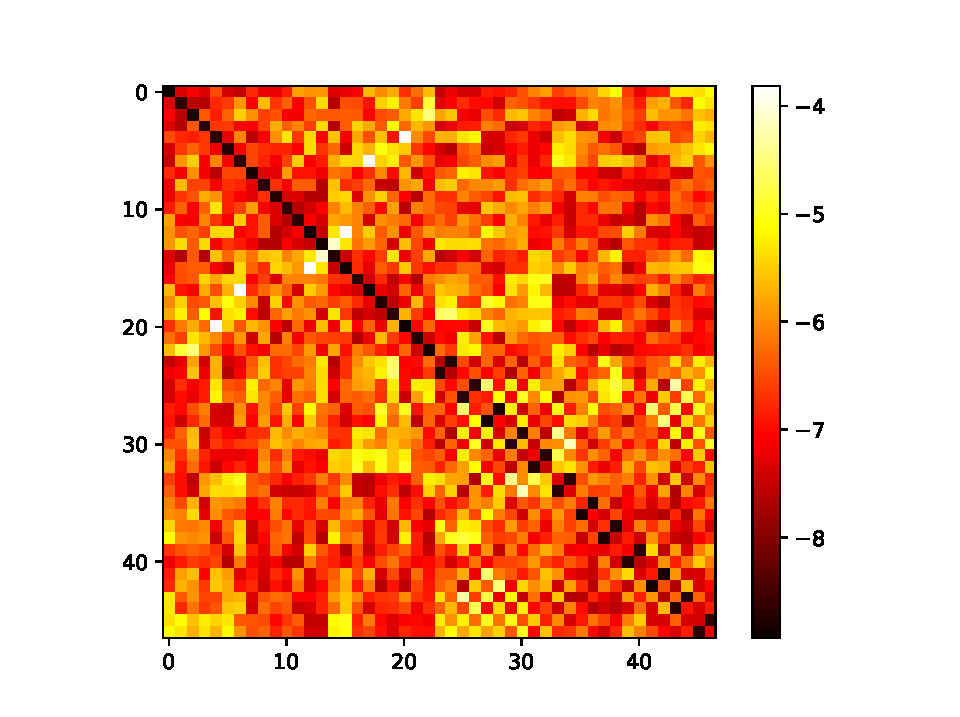
\includegraphics[width=0.7\linewidth]{interaction_matrix_full4096}
	\caption{The orthogonal set of the synthetic 4-heptad set.}
	\label{fig:interaction matrix-full4096}
\end{figure}

\section{Heuristics for building orthogonal sets}
\label{sec:heuristics}
As it can be seen from the previous sections, finding an orthogonal set as a subset of a larger set quickly becomes infeasible for long peptides. 

On the other hand, since the orthogonal subsets seem to be relatively small when compared to the sets of all corresponding peptide-pairs, we can conclude that it might be reasonable to try to algorithmically construct a smaller initial set which is likely to be ``almost orthogonal''. If we had such an algorithm, we could start constructing our set from a more convenient (from a biological point of view) set of heptads, such as the set of natural heptads.

\subsection{Greedy building}
The first heuristic that comes to mind is to generate many pairs of strongly mutually-interacting chains, and hope that we will be able to find a large orthogonal set among them. This was done in the following way:
\begin{enumerate}
	\item Choose a set of heptads (e.g. natural heptads) and the number of heptads ($k$) in all chains.
	\item Repeat the following steps to generate as many peptides as needed:
	\begin{enumerate}
		\item Choose a random strongly-interacting pair of heptads (i.e. order the heptad-pairs by interaction strength, and choose a pair from the 75th percentile). Those two heptads will be the first heptads of their respective chains.
		\item Greedily append a heptads to each chain, so as to maximize the interaction strength between them. With a small probability, we may replace these heptads with a random pair of heptads.
	\end{enumerate}
\end{enumerate}

\begin{figure}[h]
	\centering
	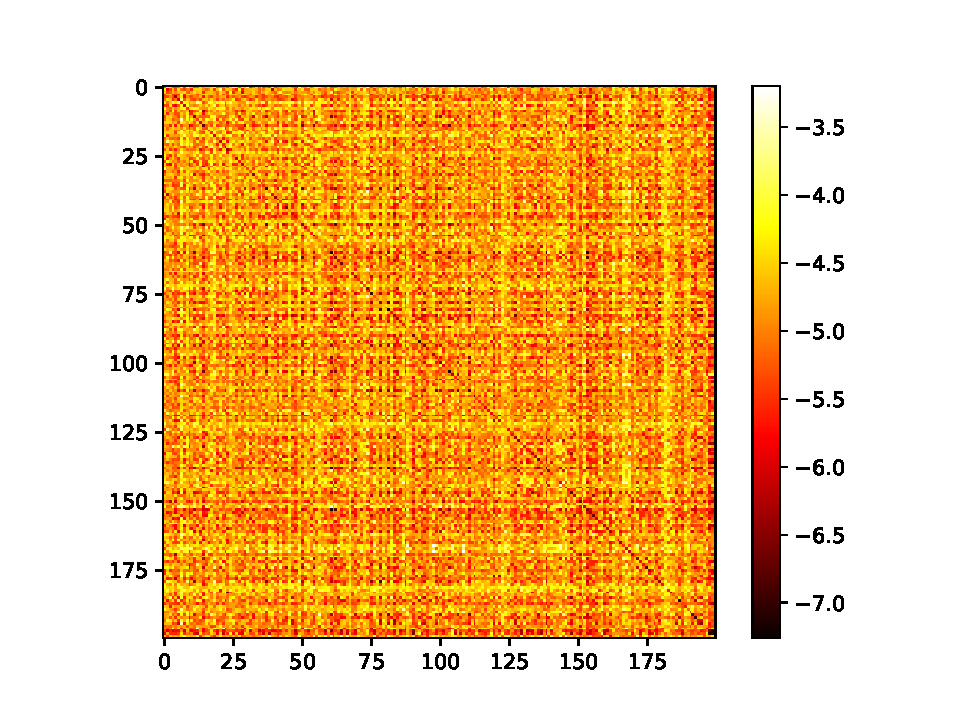
\includegraphics[width=0.7\linewidth]{interaction_matrix_greedy.pdf}
	\caption{Interaction matrix for the greedily constructed peptides.}
	\label{fig:interaction matrix-greedy}
\end{figure}

Unfortunately, as it can be seen from Figure \ref{fig:interaction matrix-greedy}, the interactions are too noisy -- instead of a clearly pronounced diagonal (desired interactions), we see many large values all around the matrix (undesired interactions). Unsurprisingly, our algorithm is unable to find a nontrivial orthogonal subset of this subset, since the obtained interaction graph was too sparse.

\subsection{Building from a short orthogonal set}
The second heuristic is to use an already-determined orthogonal set in order to build a larger orthogonal set. It turns out that it fits nicely into the intensification-diversification metaheuristics framework presented in \cite{blum2003metaheuristics}. In order to be more formal, we need the following definitions:

\begin{definition}
	Let $A$ and $B$ be peptide sets. Then, their \emph{product} $A\cdot B$ is defined as $\{ a\cdot b\: |\: a\in A, b\in B \}$, where $a \cdot b$ denotes the concatenation of sequences $a$ and $b$. Moreover, we write $A^k$ for
	$\underbrace{A\cdot A\cdots A}_{k \text{ times}}$
\end{definition}

\begin{definition}
	The \emph{length} of a peptide set $A$, denoted as $\norm{A}$, is the length of each peptide in $A$ (recall from section \ref{sec:Scoring function} that we are only considering peptide sets where all peptides have the same length).
\end{definition}
Note that the product defined above is equivalent to the usual Cartesian product of two (or more) sets, where additionally the elements of each tuple are concatenated. Moreover, from the definition of set length, we obtain $\norm{A \cdot B} = \norm{A} + \norm{B}$.

Thus, the idea is to take an orthogonal set $S_0$,  multiply it with another set $H_1$ (\emph{extension set}), and compute the orthogonal subset $S_1$ of $S_0 \cdot H_1$. The tradeoff here is that although $S\cdot H_1$ does not contain all peptides of length $\norm{S_0 \cdot H_1}$, we hope that having the product sequences start with an element of an orthogonal set will result in greater interaction specificity. Then, we proceed iteratively, by defining $S_{k+1}$ as the orthogonal subset of $S_k \cdot H_{k+1}$, until we obtain an orthogonal set of desired length. Thus, the step $S_k \to S_k \cdot H_{k+1}$ can be regarded as a \emph{diversification} step (that explores our search space), whereas $S_k \cdot H_{k+1} \to S_{k+1}$ as an \emph{intensification} step (that exploits the properties of the explored space), in the context of \cite{blum2003metaheuristics}.

One special case of this algorithm is the \emph{set squaring method}, in which $H_k = S_{k-1}$, that is, $S_{k+1}$ is the orthogonal subset of $S_k^2$. An example can be seen on Figure \ref{fig:Squaring the orthogonal set}. In it, we started with $S_0$ being the orthogonal subset of $H_r^2$, where $H_r$ is the  restricted set of $78$ natural heptads that have been observed to occur in at least $4$ different natural peptides. After that, one round of squaring is performed, to obtain $S_1$, the 4-heptad orthogonal set of $S_0^2$.
These specific sets were chosen for their length, as we will compare the end result ($4$ heptads) to the 4-heptad orthogonal set obtained from synthetic heptads. 
Unfortunately, it turns out that the starting orthogonal set $S_0$ contains only 13 peptides (Figure \ref{subfig:Interaction matrix of the natural diheptad set}). Consequently, $S_0^2$ contains only $169$ peptides, and its orthogonal set $S_1$ contains only $12$. %this is OK, S_1 is just not displayed 

Despite the disappointing results when compared to the synthetic 4-heptad set, two important insights can be made:
\begin{enumerate}
	\item The size of $S_1$ is small most likely due to lack of diversity, achieved by prematurely restricting our building blocks to just 13 orthogonal diheptads.
	\item The entries on the block-diagonal represent the peptides whose first two heptads are interacting, whereas the entries on the sub- and super-diagonals represent the peptides whose last two heptads are interacting in $S_0$. In other words, we do in fact see the positive effects of composing our peptides from elements of an orthogonal set.
\end{enumerate}

\begin{figure}[h]
	\centering
	\begin{subfigure}{0.48\linewidth}
		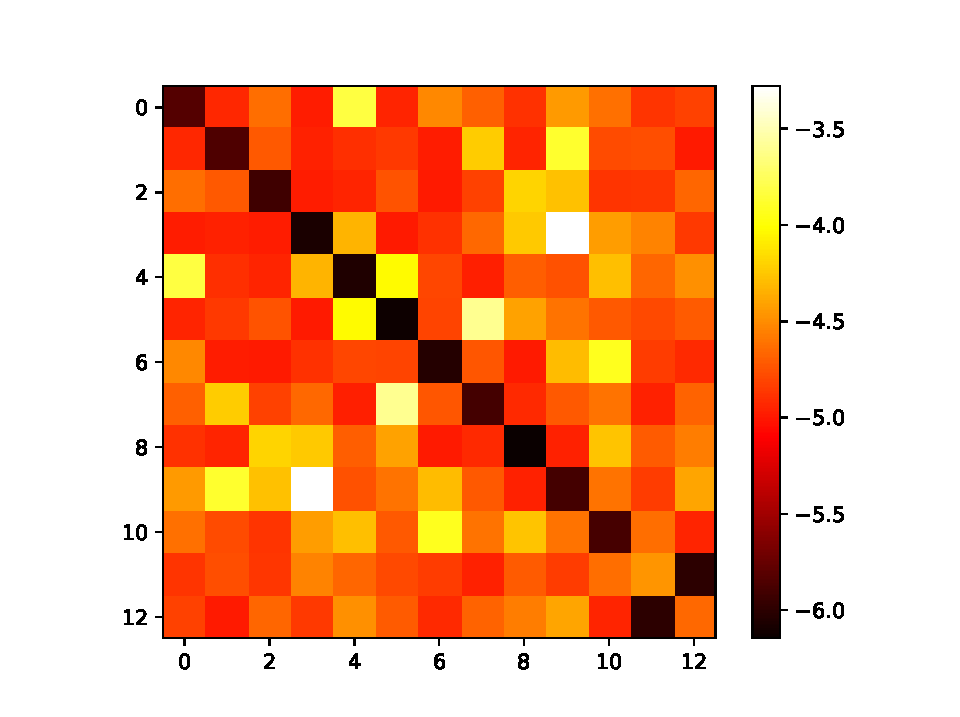
\includegraphics[width=\linewidth]{interaction_matrix_natural_diheptad_orthoset.pdf}
		\caption{Interaction matrix of orthogonal subset of the natural diheptad set.}
		\label{subfig:Interaction matrix of the natural diheptad set}
	\end{subfigure}
	~
	\begin{subfigure}{0.48\linewidth}
		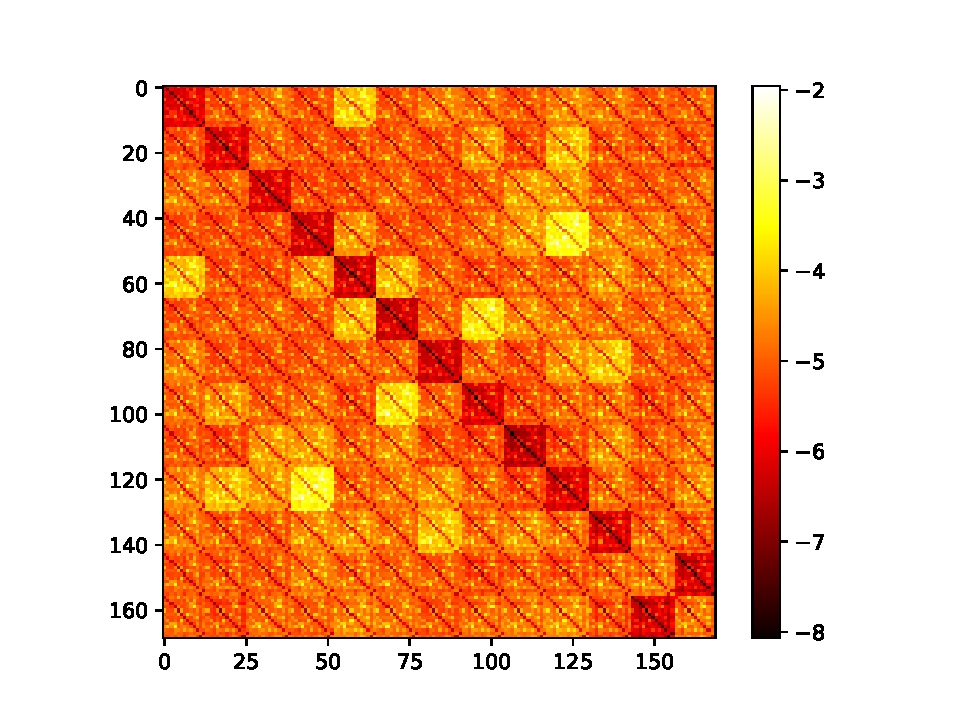
\includegraphics[width=\linewidth]{interaction_matrix_squared_natural_diheptad_orthoset.pdf}
		\caption{Interaction matrix of the square of the left set.}
		\label{subfig:Interaction matrix of the squared natural diheptad set}
	\end{subfigure}
	\caption{Squaring the orthogonal set.}
	\label{fig:Squaring the orthogonal set}
\end{figure}

Luckily, there is a way to remedy the poor results obtained by set squaring. Instead of just squaring the set at each step, we let $H_i := H$ for all $i$, where $H$ is some large set of short peptides (for example, the set of all natural heptads). In this way, we can obtain an orthogonal set composed of arbitrarily long peptides, and reintroduce some diversity at each step, by appending peptides from $H$. This result turned out to be the best among the ones listed, and for example a 104 peptide 6-heptad orthogonal set can be seen on Figure \ref{fig:interaction matrix-hexaheptad}. To our knowledge, this is most likely the largest constructed orthogonal set in published literature.

\begin{figure}[h]
	\centering
	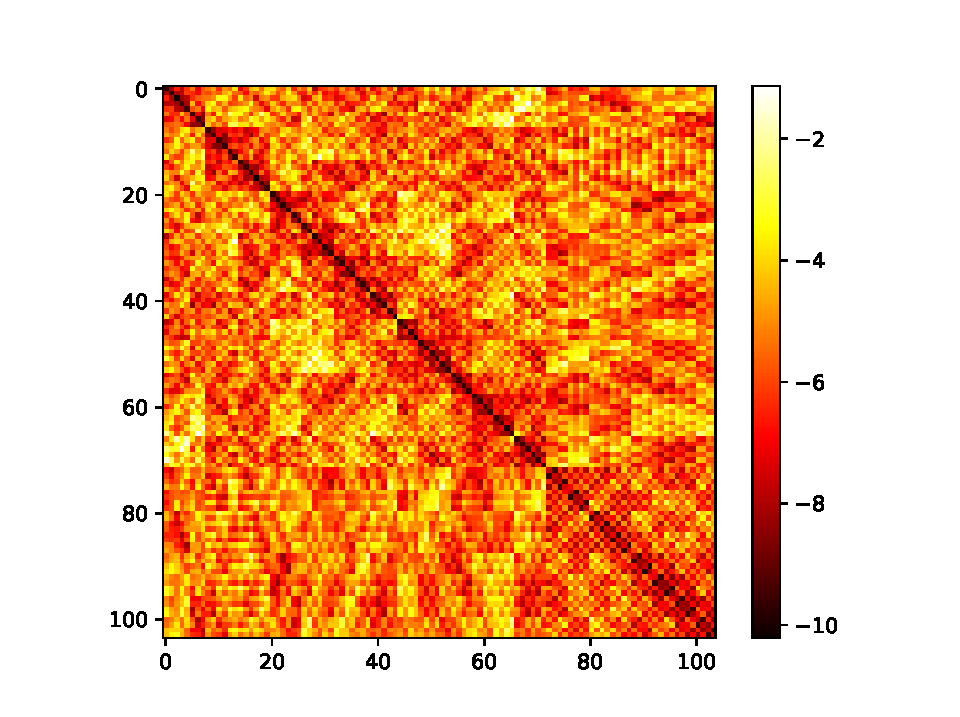
\includegraphics[width=0.7\linewidth]{interaction_matrix_hexaheptad}
	\caption{An orthogonal set built using the iterative building procedure, from the reduced set of natural heptads.}
	\label{fig:interaction matrix-hexaheptad}
\end{figure}

\chapter{Results and conclusions}
\thispagestyle{fancy}
\label{chap:Results and conclusions}

In this paper we presented the significance and theoretical underpinnings of coiled coil peptide origami, as well as novel theoretical results for constructing orthogonal sets of coiled coil dimers. In order to perform a theoretical analysis of our problem, we attempted to introduce some mathematical formalism to the field, as well as clarified the definition of an orthogonal set to include the corner case of homodimeric interactions. 

The main results are the algorithm for determining the maximum orthogonal subset of a given peptide set, as well as the iterative algorithm for building large orthogonal sets of arbitrary size. In fact, the latter enabled us to construct the largest orthogonal set of any length in known literature. Some of these orthogonal sets are currently undergoing experimental validation. It also turns out that the set-building algorithm can be described using the intensification-diversification framework for combinatorial optimization metaheuristics \cite{blum2003metaheuristics}. That result suggests that possibly even better results can be obtained by applying other metaheuristics adhering to this framework.

Apart from their practical significance, the algorithms presented can also be used in a purely theoretical setting, as heuristics for determining the distance-$d$ independent sets (first defined in \cite{agnarsson2003powers}) in certain product graphs. This area still remains to be explored in future research.

%%%%%%%%%%%%%%%%%%%%%%%%%%%%%%%%%% Summary of the final project paper in Slovene  %%%%%%%%%%%%%%%%%%%%%%%%%%%%%%%%%%%%%

\chapter{Povzetek naloge v slovenskem jeziku}
\thispagestyle{fancy}

V zadnjih nekaj desetletjih smo  dosegli pomemben napredek v našem razumevanju (bio)kemijskih procesov v živih organizmih. Posledično je vse večje  povpraševanje laboratorijev za sintetiziranje bolj zapletenih organskih molekul. Takšne molekule se nato lahko uporabijo kot podlaga za pritrditev drugih molekul ali pa kot visoko ciljno usmerjeni sistemi za dostavo delcev.

Leta 2006 so v članku \cite{rothemund2006folding} pokazali metodo zgibanja  DNA niti v 3D obliko zgolj z določitvijo nukleotidnega zaporedja. To se naredi z oblikovanjem zaporedja, tako da se nekatere njegove regije povezujejo med seboj in  po pregibanju tvorijo »žični okvir« objekta. Čeprav bi bilo zaradi bioloških razlogov koristno ponoviti slednjo  konstrukcijo z uporabo zaporedij aminokislin (peptidov, polipeptidov ali beljakovin,
odvisno od njihove dolžine), pa ni znanega nobenega računsko učinkovitega načina določanja,
ali in kako bodo peptidi v splošnem medsebojno delovali. Na srečo so  v članku \cite{potapov2015data} v posebnem primeru \emph{zvitih zvitkov} 
(ang. \emph{coiled coil} peptidov) predstavili algoritem za določanje, kako močna je interakcija med dvema takšnima peptidoma. Po drugi strani pa so v \cite{gradivsar2013design} predstavili eksperimentalne in teoretične rezultate o razredih grafov, ki jih lahko konstruiramo iz peptidne verige.

Njihov algoritem predvsem zahteva, da veriga poteka po \emph{dvojni (Eulerjevi)
poti} grafa.  Slednje porodi potrebo po veliki množici parov kratkih peptidov
(ki bodo nameščeni vzdolž povezav grafa), ki delujejo le vzajemno. Takšni množici rečemo \emph{ortogonalna množica}. Za dani interakcijski graf  $G = (V, E)$, kjer peptidi predstavljajo  vozlišča, povezave pa opisujejo prisotnost interakcije med njimi, je ortogonalna množica $S \subseteq E$ množica z naslednjima lastnostima:
\[  \{u_1,v_1\} \cap \{u_2, v_2\} = \emptyset,\] 
\[ \{u_1u_2,\; u_1v_2,\; v_1u_2,\; v_1v_2\} \cap E = \emptyset \]
za vse povezave $u_1v_1,\;u_2v_2 \in S$. Z drugimi besedami, $S$ je neodvisna množica linij\-ske\-ga grafa $L(G)$ grafa $G$ z dodatno 
omejitvijo, da nobeni dve vozlišči ne delita soseda. S prevedbo problema iskanja maksimalne ortogonalne množice v posebnem grafu na problem maksimalne neodvisne množice  pokažemo, 
da je iskanje maksimalne ortogonalne množice grafa $\NP$-težek problem. Podobno  s prevedbo na problem maksimalne neodvisne množice pokažemo, da je naš problem tudi v $\NP$, in zato $\NP$-poln. Poleg tega podamo  natančen algoritem, ki se ga lahko uporabi za določanje maksimalne ortogonalne podmnožice množice peptidov, kjer so peptidi podani z njihovimi
aminokislinskimi zaporedji. Algoritem je modificirana različica algoritma za iskanje maksimalne klike, predstavljenega v \cite{depolli2013exact}.

Prav tako predstavimo nekaj hevristik, ki izkoriščajo strukturo problema (to pomeni,
da grafi, ki jih obravnavamo, niso splošni grafi, ampak so zgrajeni iz uteženih peptidnih
interakcijskih grafov) za konstrukcijo večje ortogonalne množice. 
Natančneje, predstavljena sta dva požrešna pristopa:
\begin{enumerate}
	\item neposredna konstrukcija parov po možnosti močnejših interakcijskih verig in določitev
	njihove maksimalne ortogonalne podmnožice in
	\item iterativna razširitev  manjše ortogonalne množice  z alternativno uporabo njenega kartezijskega produkta z drugo množico in določitev maksimalne ortogonalne podmnožice 
	(še zmerno velikega) dobljenega produkta.
\end{enumerate} 
Opozorimo, da slednji pristop porodi ortogonalne množice, ki so 3 do 10 krat večje od tistih, ki jih dobimo z natančnimi metodami kot podmnožice manjših množic.
Dobljeni rezultati so za zdaj med najboljšimi v literaturi.

Nazadnje omenimo še  možne uporabe nove  od spodaj navzgor  zasnovane hevristike za reševanje problema maksimalne ortogonalne množice na splošnih grafih.

%%%%%%%%%%%%%%%%%%%%%%%%%%%%%%%% Bibliography %%%%%%%%%%%%%%%%%%%%%%%%%%%%%%%%%

\thispagestyle{fancy}

\bibliographystyle{plain}
\bibliography{bibliography}

\label{LastPage} 
\phantom{dummy}

\end{document}
